


\begin{figure}[ht]
\centering
\includegraphics[width=0.8\textwidth]{./chapters/demonstration/base/mcI.eps}
\caption[$^{235}U$ residence. Mixed Cell Sorption Limitation Without Solubility Limitation.]{
For the MCI case in which total containment is only is assumed in the far field, 
but sorption and solubility limitation neglected, demonstrates results exactly similar to 
DRIV, as expected.}
\label{fig:mcI}
\begin{minipage}[b]{0.45\linewidth}

  \includegraphics[width=\textwidth]{./chapters/demonstration/base/mcI1.eps}
  \caption[MCI Waste Form Contaminants.]{
    Waste Form 5 ($F_d = 0.1$) releases material with degradation. 
    }
  \label{fig:mcIwf5}
  
  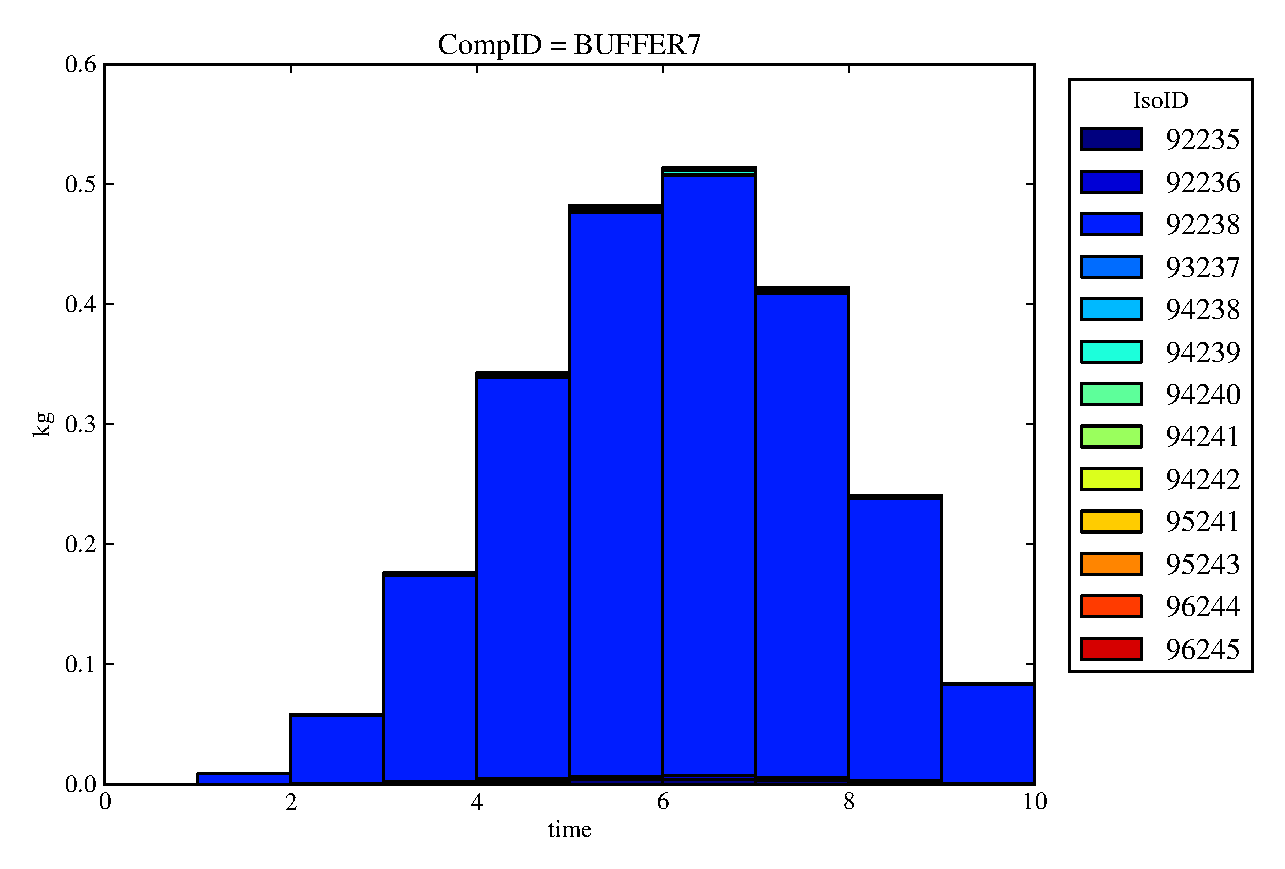
\includegraphics[width=\textwidth]{./chapters/demonstration/base/mcI3.eps}
  \caption[Case MCI Buffer Contaminants]{
    The Buffer, component 7 ($F_d=0.1$), receives then releases material.
    }
  \label{fig:mcIbuff}

\end{minipage}
\hspace{0.05\linewidth}
\begin{minipage}[b]{0.45\linewidth}
  \includegraphics[width=\textwidth]{./chapters/demonstration/base/mcI2.eps}
  \caption[Case MCI Waste Package Contaminants.]{ 
    Waste Package 6 ($F_d = 0.1$) recieves then releases material.
    }
  \label{fig:mcIwp6}

  \includegraphics[width=\textwidth]{./chapters/demonstration/base/mcI0.eps}
  \caption[Case MCI Waste Package Contaminants.]{ 
    The Far Field, component 4 ($F_d = 0.0$), acheives full containment.
    }
  \label{fig:mcIff0}


  \end{minipage}
\end{figure}

\begin{figure}[ht]
\centering
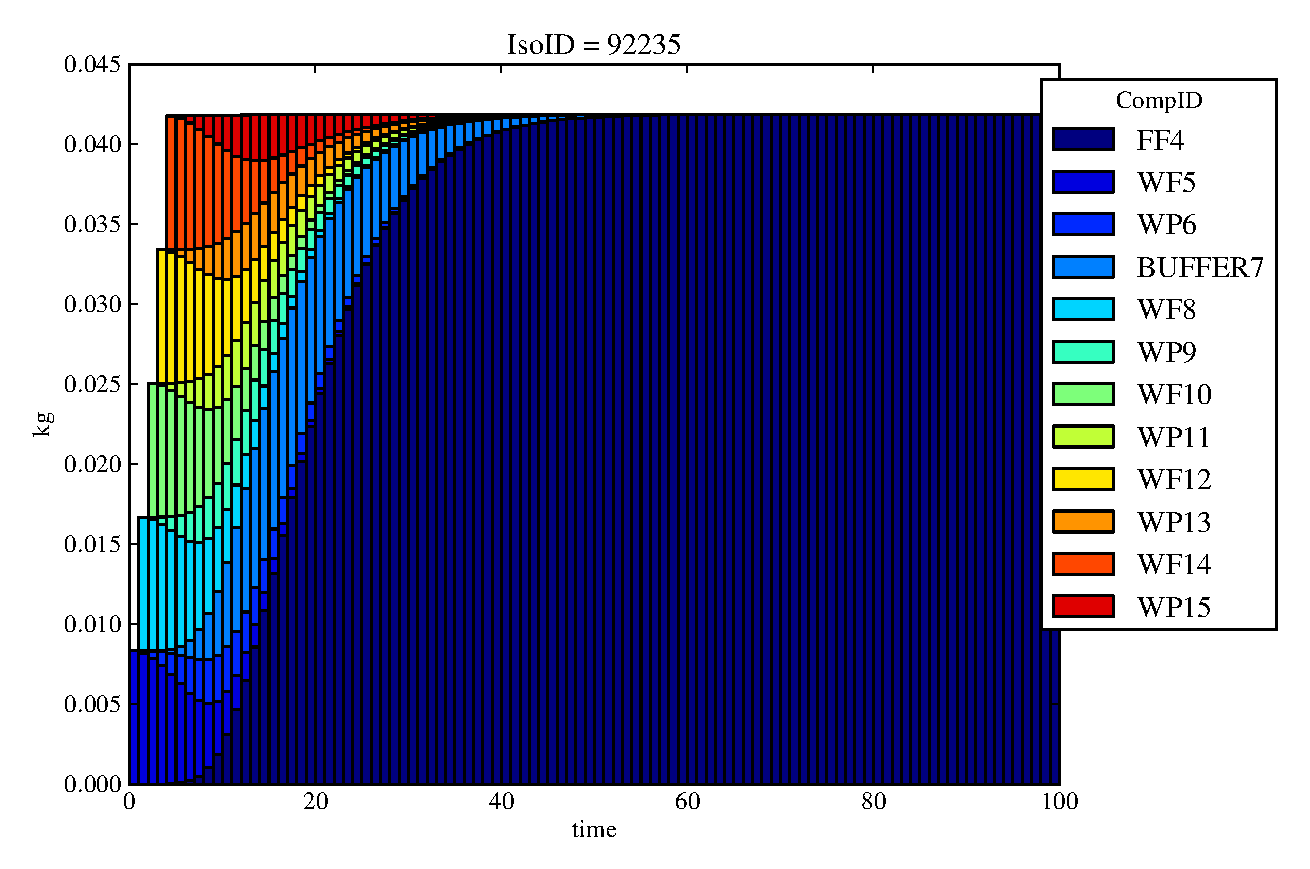
\includegraphics[width=0.8\textwidth]{./chapters/demonstration/base/mcIII.eps}
\caption[$^{235}U$ residence. Mixed Cell Coupled Sorption and Solubility Limitation.]{
For the MCII case in which containment is affected by both sorption and solubility limitation, 
($F_{d}=0.1$ for all components), $^{235}U$ travels more slowly than in the MCI case 
before permanent residence in the far field component.
}
\label{fig:mcIIIall}
\begin{minipage}[b]{0.45\linewidth}

  \includegraphics[width=\textwidth]{./chapters/demonstration/base/mcIII1.eps}
  \caption[MCI Waste Form Contaminants.]{
    Waste Form 5 ($F_d = 0.1$) releases material with degradation. 
    }
  \label{fig:mcIIIwf5}
  
  \includegraphics[width=\textwidth]{./chapters/demonstration/base/mcIII3.eps}
  \caption[Case MCI Buffer Contaminants]{
    The Buffer, component 7 ($F_d=0.1$), receives and then releases material.
    }
  \label{fig:mcIIIbuff}

\end{minipage}
\hspace{0.05\linewidth}
\begin{minipage}[b]{0.45\linewidth}
  \includegraphics[width=\textwidth]{./chapters/demonstration/base/mcIII2.eps}
  \caption[Case MCI Waste Package Contaminants.]{ 
    Waste Package 6 ($F_d = 0.1$) recieves then releases material. 
    }
  \label{fig:mcIIIwp6}

  \includegraphics[width=\textwidth]{./chapters/demonstration/base/mcIII0.eps}
  \caption[Case MCI Waste Package Contaminants.]{ 
    The Far Field, component 0 ($F_d = 0.1$), acheives total containment.
    }
  \label{fig:mcII}


  \end{minipage}
\end{figure}

